\section{Results}

\subsection{Heat technology generation on the sub-region (NUTS3) level}
\textcolor{magenta}{Vier verschiedene Bilder von den vier Storylines zeigen. Eventuell sieht man, dass in den dichtbesiedelten Gebieten dann eher unabhängig von der Storyline entsprechend Technologien dominieren.}

Hier kommt ein grouped bar plot mit den Regionen die network haben und stacked in zwei komponenten nämlich network-based und nicht network-based. 

%\begin{figure}[h]
%	\centering
%	\includegraphics[width=1\linewidth]{figures/4_Results/Directed_Transition.eps}
%	\caption{}
%	\label{fig:res1}
%\end{figure}


\begin{sidewaysfigure}
	\centering
	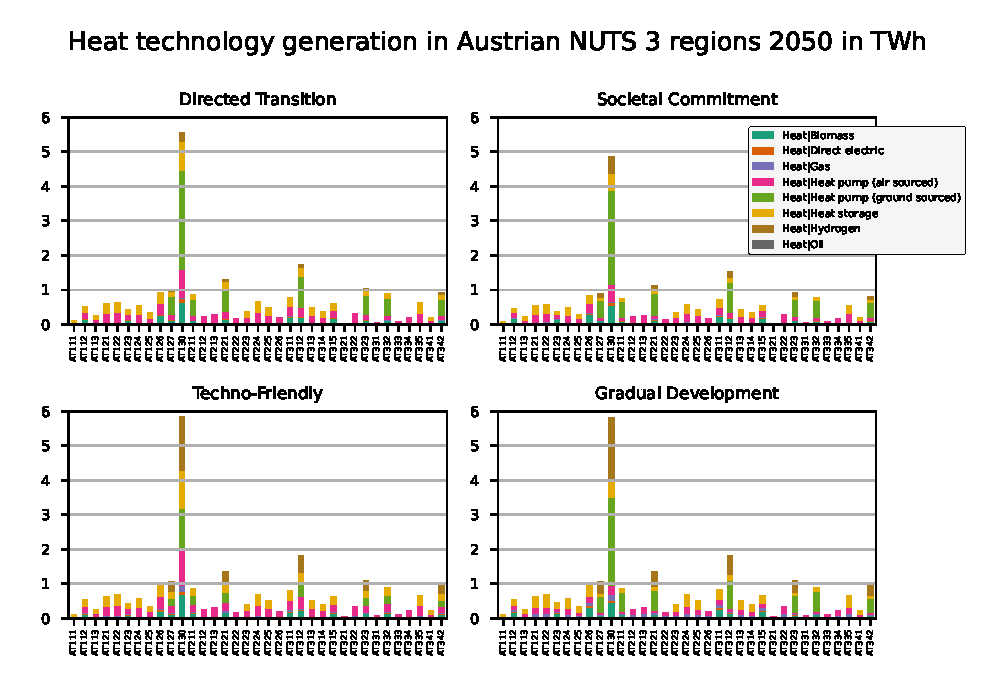
\includegraphics[width=1\linewidth]{figures/4_Results/NUTS3.eps}
	\caption{}
	\label{fig:res1}
\end{sidewaysfigure}

\begin{sidewaysfigure}
	\centering
	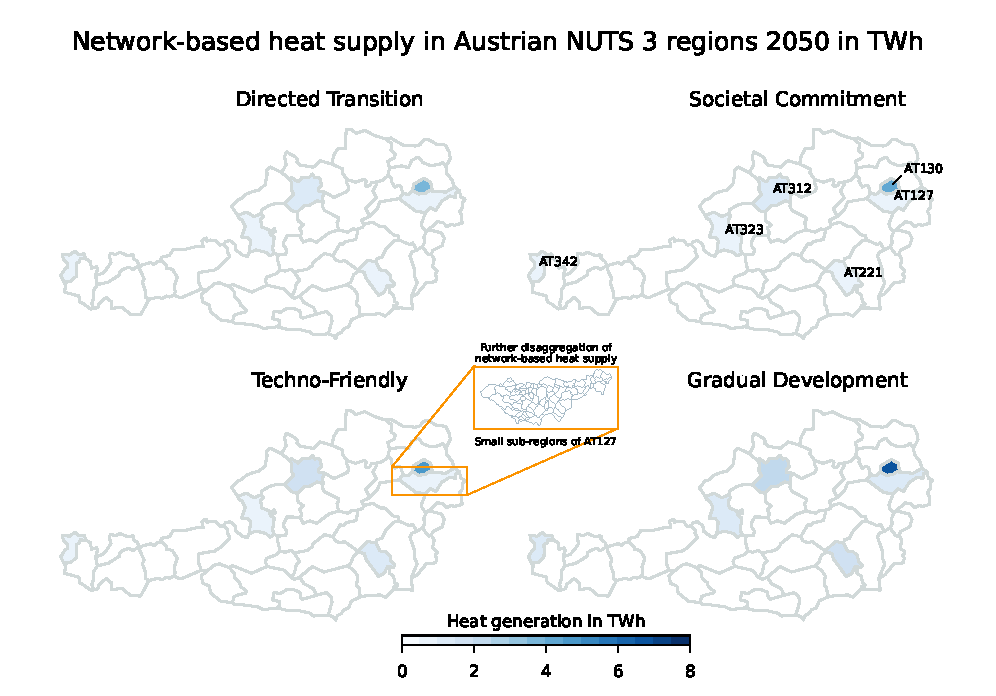
\includegraphics[width=1\linewidth]{figures/4_Results/Heatmap.eps}
	\caption{}
	\label{fig:res2}
\end{sidewaysfigure}
